\cleardoublepage
%To do notes colors meaning
%red - Not started
%yellow - In progress
%light blue - Done, under approval
%Green - Done and approved
\chapter{State of the Art}%\label{chap:stArt}
%%Section To do
\todo[inline,color=blue!40]{*1-The LPG cylinder}
\todo[inline,color=yellow!40]{*2-Measuring/Stimulation Tecniques}
\todo[inline,color=yellow!40]{*3-Signals and systems - missing images}
\todo[inline,color=red!40]{*4-LPG cylinder Model}


%----------------------------------------Section 1-----------------------------------
\section{The LPG cylinder}
%Subsections to do
\todo[inline,color=yellow!20]{*Integrate all}
The LPG cylinders commonly used in house appliances, usually came in different weight types, that are change according to the cylinder construction, the supplier, his application and composition of gas that is being healed inside the container. One thing that is similar is the state of the gas under certain circumstances, for instance the boiling point of LPG is around -42ºC, which means that under ambient pressure/temperature the gas is in his gaseous state. 

Usually inside a LPG cylinder, the gas is kept in a liquid and gas form, in a percentage of around 80\% and 20\%, respectively, with a constant pressure, this percentage allows, when the external temperature rises, affecting the internal temperature, for both gas and liquid to expand until a certain limit, without compromise the safety of the use of the cylinders.
\begin{figure}[!htb]
    \centering
    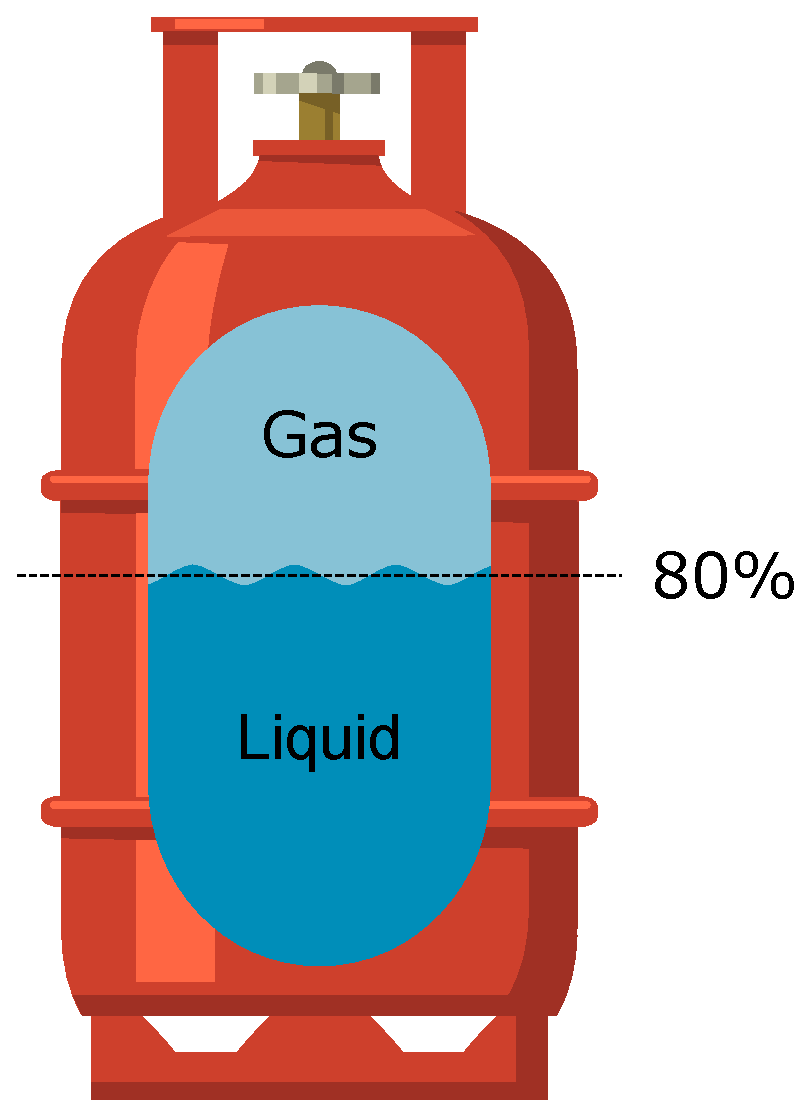
\includegraphics[width=0.25\textwidth]{Chapters/2CHP/Diagrams/bottleBaseliqGas.eps}
    \caption{LPG cylinder internal state composition}
    \label{fig:intcomplpg}
\end{figure}

When the cylinders are empty and need to be filled, there is a direct relation between the amount of pressure, needed to fill the cylinders, and the temperature of the gas, the higher the temperature of the gas the higher is the pressure needed to fill the cylinder, this process of turning the LPG in a gas form into a liquid by pressurizing it, is called liquefaction. Another relation that must be taken into consideration, is the weight of the cylinder and the amount of liquid LPG, when the cylinder valve is open and LPG gas is released, the liquid LPG is turns into gas in order to keep a balance of pressure inside the cylinder, since that for the same pressure the density of the LPG liquid is higher then the density of the LPG gas, when the amount of liquid LPG decreases the weight of the cylinder also decreases \cite{WhatAreProperties} \cite{PropaneDensitySpecific}.

%%Correct about gas pressure inside the bottle

%----------------------------------------Section 2-----------------------------------
\section{Measuring/Stimulation Techniques}
\subsection{Measuring Techniques}
As the LPG cylinder content is divided in two physical states, liquid and gaseous, over the years several techniques have been used and improved in measuring the liquid level, which is how is determined the amount of LPG in the cylinder, some of the different techniques used are based on the same method. Those methods are usually split in two different categories, contact and contactless. Contact measuring methods usually include, mechanical, electrical or pressure sensing devices. In this methods the sensors are in direct contact with the liquid. In contactless, the methods used usually are more complex to process, when compared with contact methods. In this case the methods of measuring are mainly through optical, ultra-sound, vibration and weight analysis\cite{nakagawaContactlessLiquidLevelMeasurement2013a}. 
\todo[inline,color=yellow!40]{*format correctly}
\begin{figure}[!htp]
    \centering
    \begin{subfigure}{0.15\textwidth}
        \centering
        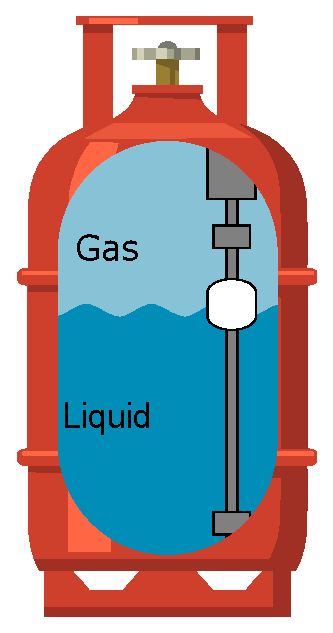
\includegraphics[width=\linewidth]{Chapters/2CHP/Diagrams/bottleBasefluctuator.eps}
        \caption{}
        %\label{subfig:g1lines}
    \end{subfigure}
    \begin{subfigure}{0.15\textwidth}
        \centering
        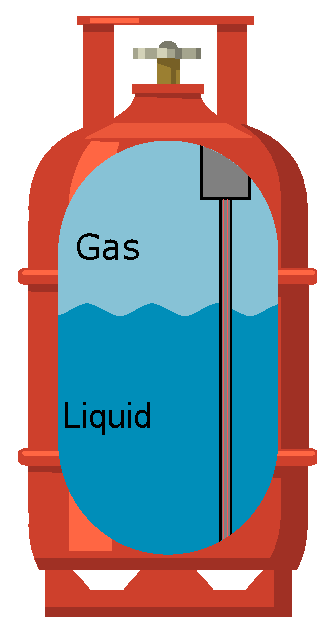
\includegraphics[width=\linewidth]{Chapters/2CHP/Diagrams/bottleBaseelectrode.eps}
        \caption{}
        %\label{subfig:g2lines}
    \end{subfigure}
    \begin{subfigure}{0.15\textwidth}
        \centering
        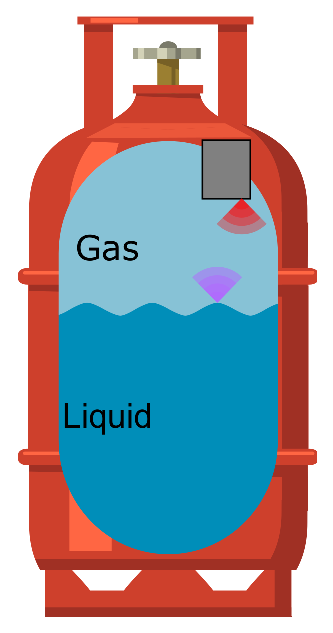
\includegraphics[width=\linewidth]{Chapters/2CHP/Diagrams/bottleBaseultrasound.eps}
        \caption{}
        %\label{subfig:g3lines}
    \end{subfigure}
    \begin{subfigure}{0.15\textwidth}
        \centering
        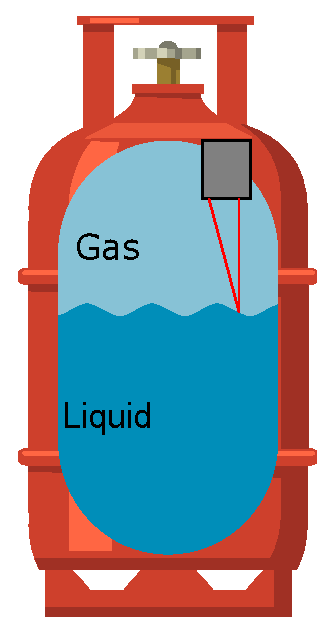
\includegraphics[width=\linewidth]{Chapters/2CHP/Diagrams/bottleBaseoptical.eps}
        \caption{}
        %\label{subfig:g4lines}
    \end{subfigure}
    \caption{Different LPG cylinder to used to compare the relation between Frequency and Weight for different models\citeauthor{wuLiquidLevelDetector2014b}}
     %\label{fig:noise}
 \end{figure}
Taking in consideration the fact that a LPG cylinder is opaque and isolated, some of the methods can't be used in the process, for instance, a mechanical float-type isn't a suitable solution to use inside the cylinder, or in the same way to use an electrode, as a electrical method, in these cases the device would require to be installed inside the cylinder during his fabrication process, possibly implying the substitution of the current cylinders. In the same way, in contactless methods, the use of different optical techniques and the use of of ultra-sound, would face the same problem mentioned with the contact methods, being also discard as a suitable method in this situation. 

From previous research, some work has already been developed with the purpose of measuring the amount of liquid gas inside a LPG cylinder. Being the techniques used based on the methods presented above.
%Based on the pressure
\todo[inline,color=blue!20]{*Pressure based device}
In a work from \citeauthor{baigAccurateMeasurementPressure2008b} a pressure sensing device was developed, with the final appliance to a LPG cars, but with the possibility of apply in other circumstances. The device uses the pressure variation to move a magnet and using a Hall Effect sensor, with a fixed position, this motion produces a linear change of the voltage in the sensor, giving an accurate method of measuring the amount of gas in the LPG cylinder, in this case\cite{baigAccurateMeasurementPressure2008b}. 
%Based on the weight
\todo[inline,color=blue!20]{*Weight device}
A common method of evaluate the amount of gas inside a LPG cylinder, is based on the weight change of the cylinder, that decreases with the consumption of liquid gas. As an example, the work developed by \citeauthor{dasilvamedeirosSmartgasSmartPlatform2017a}, \citeauthor{shresthaIoTBasedSmart2019a} or \citeauthor{shinganSmartGasCylinder2017a} have similar approaches to measure the amount of liquid gas inside the LPG cylinder, since it's quite simple to implement, for a simply measure it only requires a load cell, a amplifier and a microcontroller to display the result. This technique is also very precise, if there isn't a huge temperature change, that would affect the density of the liquid gas\cite{dasilvamedeirosSmartgasSmartPlatform2017a}\cite{shresthaIoTBasedSmart2019a}\cite{shinganSmartGasCylinder2017a}.
Several works have been developed based on this technique, since it only requires a load cell and a microcontroller
%Based on Wave analysis
\todo[inline,color=blue!20]{*Waves based device}
Another method used that proved to be valid for measuring the amount of liquid inside a closed and opaque container, is based on the analysis of the vibrations. A container filled with liquid, produces different sounds for different types of liquids or their variation. As a example of an implementation based on this principles is the work of \citeauthor{jahnLevelSensorFluids2014a} or \citeauthor{wuAnalysisImplementationNoncontact2016a}, both cases evaluate the vibration of the liquid inside the LPG cylinder, but they have a different approach. In the first case the level is measured by correlate a signal with a known frequency with another obtained from direct measurement from the cylinder, the known signal is used as an indirect impulse in the cylinder, by continuously change the frequency of this signal and correlate it with the captured signal, the dominant frequency is found when the highest correlation is found. In the second case is much simpler the implementation, a device knocks on the cylinder and the measured signal is processed with a FFT. In both cases the frequency obtained corresponds to a certain level o liquid, being a downside the fact that for a different container, a recalibration is necessary\cite{jahnLevelSensorFluids2014a}\cite{wuAnalysisImplementationNoncontact2016a}. 

To the purpose of this dissertation, the approach of \citeauthor{wuAnalysisImplementationNoncontact2016a} is being reproduce, by implementing it in a microcontroller, capable of process the resulting vibration caused by knocking in the LPG cylinder. 
\subsection{Stimulation Techniques}
\todo[inline,color=red!40]{Stimulation Tecniques}

%----------------------------------------Section 3-----------------------------------

\section{Signals and System}

\todo[inline,color=yellow!40]{*1-Vibration}
\todo[inline,color=yellow!40]{*2-Signal definition}
\todo[inline,color=yellow!40]{*3-Signal and Digitalization}
\todo[inline,color=yellow!40]{*4-System definition}
\todo[inline,color=yellow!40]{*5-LTI Systems}
\todo[inline,color=yellow!40]{*6-Discrete-Time Fourier-Transform}

\subsection{Vibration}
The vibration and the studies in this field are usually related with the oscillatory motion of a body and the forces associated with them. Bodies with mass and elasticity are capable of experience vibration, knowing that, for example, when a structure is design, is required to take in consideration the oscillatory behavior of the structure. There are two types of vibration, free and forced. The first takes place when a system oscillates under forces natural to the system itself and there is no action of external forces. Under free vibration the system will vibrate at one or more of its natural frequencies, stablished by the properties of the system. Forced vibration occurs when the system is under the excitation of external forces. If it oscillatory, the system will vibrate at the same frequency of the external oscillation, if this frequency matches one of its natural frequencies a resonant state is reached, which may dangerous for a structure stability.   

\subsection{Signal definition}
Signals can describe a large variety of physical phenomenon's, bringing a certain information about it, depending of the phenomenon represented. For example, the voltage variation in a capacitor, or the human voice which creates variations in acoustic pressure, captured by a microphone that senses those variations and convert them into a electrical signal. A signal can be represented mathematically as a function of one or more independent variables. 
To what concern in signal processing, the types of signal considered are two types, continuous-time signals and discrete-time signals. In these cases, the independent variable is continuous and discrete, respectively\cite{oppenheimSignalsSystems1997}.

\subsection{Signal and Digitalization}
A continuous-time signal can be represented in a discrete-time form by the knowledge of its values at certain points in time equally spaced. This is called sampling theorem, and if the samples are close to each other, less time between samples, the more similar the discrete signal became to the continuous. Sampling plays an important role between the continuous-time and the discrete-time.

Considering a continuous-time signal $x(t)$ is measured at every $T$ seconds. The is discretized in units of the sampling interval $T$:
\begin{center}
    $t = nT_s,\> n = 0, 1, 2, ...$
\end{center}
The variable $T$ is called sampling period and the inverse of the period $f_s=\frac{1}{T}$ being the sampling frequency. One of the problems of this conversion is usually related with the correct choose of the sampling period, for that the theorem clearly specifies that the sampling period must be small enough so if there are small variations in the signal, they don't get lost between samples. Therefor the theorem says that the sampling frequency $f_s$ must be chosen to be  at least twice the maximum frequency $f_{max}$. A continuous-time signal $x(t)$ is bandlimited, so its frequency spectrum is limited at maximum frequency $f_{max}$, and no frequencies above that.

\begin{equation} \label{eq:sampFreq}
       f_s \geq 2f_{max}
\end{equation}
\begin{equation} \label{eq:sampPeriod}
    T \leq \frac{1}{2f_{max}}
\end{equation}

The minimum value of the sampling frequency allowed by the theorem, is called the Nyquist rate, and his value is $f_s = 2f_{max}$. Oppositely, for a known value of $f_s$ the maximum frequency of the signal is $f_{max}=\frac{f_s}{2}$ and is called the Nyquist frequency of folding frequency.

For the representation of some signals is usually used a unit impulse as a method to build a block to represent and construct other signals. The simplest representation of a unit impulse (or unit sample), in discrete-time, is defined as follows:
\begin{equation}
    \delta[n] = \left\{ \begin{matrix} 
    0, n \ne 0\\
    1, n = 0\\
    \end{matrix}\right.
\end{equation}
Another example of a simple discrete-time signal is the unit step, defined as:
\begin{equation}
    u[n] = \left\{ \begin{matrix} 
    0, n < 0\\
    1, n \geq 0\\
    \end{matrix}\right.
\end{equation}
If a close analysis is made, is possible to conclude that there is a relation between a unit impulse and a unit step, a unit step can be represented as a sum of impulses
\begin{equation}\label{eq:step}
    u[n] = \sum_{k=0}^{\infty}\delta[n-k]
\end{equation}
The equation \ref{eq:step} can be seen as a sum of delayed impulses and plays an important role in the sampling property.\\
The values of the $f_{max}$ and $f_s$ depend on the application, and the Nyquist frequency usually defines the cutoff frequencies used in filters required in DSP applications. A example of the of the typical sampling rates of common DSP applications are shown in the following table:   
\begin{table}[!htpb]
   \centering
   \begin{tabular}{|c|c|c|} \toprule
       {application}&{$f_max$}&{$f_s$}\\
       \toprule
       {geophysical}&{500 Hz}&{1 kHz}\\
       {biomedical}&{1 kHz}&{2 kHz}\\
       {mechanical}&{2 kHz}&{4 kHz}\\
       {speech}&{4 kHz}&{8 kHz}\\
       {audio}&{20 kHz}&{40 kHz}\\
       {video}&{4 MHz}&{8MHz}\\
       \bottomrule
   \end{tabular} 
   \caption{Common sampling rates per application\cite{orfanidisIntroductionSignalProcessing1996}}  
    \label{tab:sampRat}     
\end{table} 

\subsection{System definition}\label{subsec:SysDef}
There is no specific nature to a system, and there is vast example of systems all around us, they could be biological, mechanical, electrical, among others. In the signal processing context a system can be viewed as a process in which input signals are transformed by the system or cause the system to respond in some way, with the resulting in new output signals. Simplifying, a system can be described as an entity with a specific function, where the output signal is the result of the manipulation one or more input signals.
To the types of signals mentioned, continuous and discrete, the systems usually are represented as in the \ref{eq:systemeq}, in both cases $x$ represents input and $y$ output.
\begin{equation} \label{eq:systemeq}
    \begin{split}
        y(t) = H[x(t)] \\
        y[n] = H[x[n]]
    \end{split}
\end{equation}

One of the motivations for the study/analysis of systems from various applications, thus systems from different applications, with similar behavior, can have similar mathematical descriptions. The description of a system as a mathematical function also allows to simulate the behavior in a certain application, testing the response of it with different techniques. 

A system can be described with certain properties, each one having a different effect on the system output. The properties are stability, memory, causality, invertibility, time-invariance and linearity. In signal-processing context, invertibility and time-invariance have special relevance, with a profound study of linear time-invariant(LTI) systems further ahead.\cite{oppenheimSignalsSystems1997}
\subsubsection*{Stability}
A system is considered stable if an input signal limited in amplitude, results in a output signal also limited in amplitude. The system operation, H, is stable if the output signal $y(t)$  satisfies the following condition
\begin{equation}
    |y(t)|\leq M_y < \infty , \forall t
\end{equation}
If the input signal $x(t)$ satisfies the condition
\begin{equation}
    |x(t)|\leq M_x < \infty , \forall t
\end{equation}
The values of $M_x$ and $M_y$ correspond to finite positive numbers. The conditions for the stability of a discrete-time system can be described in the same way.
\subsubsection*{Memory}
A system has memory, when the output signal depends on past values of the input signal. The temporal extension of the past values on which the output depends, defines how far the memory of the system extends. One example of a system with memory is the current $i(t)$ in a inductor and the relation of his voltage $v(t)$:
\begin{equation}
    i(t)=\frac{1}{L}\int_{-\infty}{t}v(\tau)d\tau
\end{equation}
For a discrete-time system, the conditions are similar. 
\subsubsection*{Causality}
A system is considered \textit{causal} if his resulting output signal, only depends in present/past values of the input signal. Opposed to that, a \textit{noncausal} system can have is output depending on future values of the input signal.
An example of a \textit{causal} output is the following:
\begin{equation}
    y[n] = \frac{1}{3}(x[n+1]+x[n]+x[n-1])
\end{equation}
On the other hand an example of a \textit{noncausal} is:
\begin{equation}
    y[n] = \frac{1}{3}(x[n]+x[n-1]+x[n-2])
\end{equation}
\subsubsection*{Invertibility}
A system is considered invertible if is possible to recover the input from the output signal of the system. The operation to recover the signal may be a different system connected to the output of the first. If the operation of a system is represented with $H$ in a continuous-time domain, with $x(t)$ and $y(t)$ being the input and output, respectively. The $y(t)$ is applied to the second system, where the result is expected to be $x(t)$, as follows:
\begin{equation}
    \begin{aligned}
        H^{-1}{y(t)} = H^{-1}{H\{x(t)\}}\\
        = H^{-1}H\{x(t)\}    
    \end{aligned}
\end{equation} 
As the $H^{-1}H$ denotes the identity operation. If $H^{-1}$ is the inverse operation of the $H$ then the output of the second operation is the same as the input of the first operation. This property has special relevance in the design of communications systems. 

\subsubsection*{Time-Invariance}
A system is considered time invariant if a time delay in the input signal, results as well in a delay of the output signal. This means that a certain system will respond in the same way, whenever a signal is applied in input, meaning that the characteristics of the system won't change with time. Considering a continuous-time system, with $x(t)$ and $y(t)$ being the input and the output, respectively. Represented as follows:
\begin{equation}
    y(t) = H\{x(t)\}
\end{equation} 
If the input signal is delayed by $t_0$ seconds, the new input signal is $x(t-t_0)$ and an be described as follows:
\begin{equation}
    x(t-t_0) = S^{t_0}\{x(t)\}
\end{equation}
Where the $S^{t_0}$ represents the delay. So the new output signal $y_i(t)$, resulting from the delay applied in the will be:
\begin{equation}
    \begin{aligned}
        y_i(t) = H\{x(t-t_0)\}\\
        = H\{S^{t_0}\{x(t)\}\}\\
        =HS^{t_0}\{x(t)\}    
    \end{aligned}
\end{equation}
Now considering $y_o$ the output signal of the original system delayed by $t_0$ seconds: 
\begin{equation}
    \begin{aligned}
        y_i(t) = S^{t_0}\{y(t)\}\\
        = S^{t_0}\{H\{x(t)\}\}\\
        =S^{t_0}H\{x(t)\}    
    \end{aligned}
\end{equation}
The system is time invariant if the outputs are equal for an identical input signal $x(t)$. 
\begin{equation}
    HS^{t_0} = S^{t_0}H
\end{equation}
This means that, for a system $H$ to be time invariant, the system $H$ and the time delay $S^{t_0}$ must commute with each other for $t_0$. A similar relation in the discrete-time system to be time invariant.  
\subsubsection*{Linearity}
A system is considered \textit{linear} if fills all the requirements of the \textit{principle of superposition}. That is, if the response of a system to a weighted sum of input signals is equal to the same weighted sum of the output signals, in each one of the output signals being the result of a certain input signal acting independently in the system. If this principle is not fulfilled, the system is called \textit{nonlinear}. 
A weighted sum of continuous-time signals: 
\begin{equation}
    x(t) = \sum_{i=1}^{N}a_ix_i(t)
\end{equation}
Is applied to a system $H$, where $a_1, a_2, ..., a_N$ correspond the weight factor and $x_1(t), x_2(t), ..., x_N(t)$ correspond to the input signals. Resulting in the system response as represented:
\begin{equation}
    \begin{aligned}
        y(t) = H\{x(t)\}\\
        =H\{\sum_{i=1}^{N}a_ix_i(t)\}\\
    \end{aligned}
\end{equation} 
If the system is linear then, the weighted sum of output signals is:
\begin{equation}
    \begin{aligned}
        y(t) = \sum_{i=1}^{N}a_iy_i(t)\\
        y_i(t) = H\{x_i(t)\}   
    \end{aligned}
\end{equation}
This result in
\begin{equation}
    y(t) = \sum_{i=1}^{N}a_i H\{x_i(t)\}    
\end{equation}
which is the equivalent mathematical representation as in a weighted sum of inputs. To represent them in the same form, the system operation can commute with the amplitude and sum scaling. This principle also applies to discrete-time systems in a similar form. 


\subsection{LTI Systems} \label{subsec:LTI}
As systems can be found all around us, so does a LPG bottle can be considered as a system. If the mathematical model that represents it meet the last two properties mentioned, it can be referred as a linear time-invariance (LTI) system. These properties combined with the characteristics of the unit impulse, being able to represent common signals as a representation of combined delayed impulses, this allows to completely characterize a LTI to what referrers his impulse response.\cite{oppenheimSignalsSystems1997}
Similar to a unit step $u[n]$, a common signal $x[n]$ can be represented by unit impulses, as follows:
\begin{equation}
    x[n] \sum_{k=-\infty}^{+\infty} x[k]\delta[n-k]
\end{equation}
In this case the weights in the linear combination are $x[k]$. Another aspect to take in consideration in these types of systems, is the response of the system to a impulse $\delta[n]$, results in $h[n] = H[\delta[n]]$. With this in mind, the response of a linear system $y[n]$ to a common input signal $x[n]$, represented from a combination of shifted impulse, can be represented as:
\begin{equation}
    \begin{matrix}
        y[n] & = & H\big[x[n]\big] \\
        \ & = & \sum_{k=-\infty}^{+\infty} x[k]h[n-k]
    \end{matrix}
\end{equation}
The result is known as the \textit{convolution sum} or \textit{superposition sum} and the operation as \textit{convolution} of the sequences $x[n]$ and $h[n]$. The operation can be represented as:
\begin{equation}
    y[n] = x[n] * h[n]
\end{equation} 
\subsection{Discrete-Time Fourier-Transform}
For the analysis of LTI systems, one of the most powerful and used tools is the Fourier-Series and Fourier Transform. For the analysis purpose, the focus is only going to be the Discrete-Time Fourier-Transform (DTFT). The study of this type of systems offers two great advantages:
\begin{itemize}
    \item It is possible to construct a extensive and convenient class of signals, based on a set of simpler signals.
    \item The response of the LTI signal should be simple enough, to provide a convenient representation of the response from the system to any signal based on the combination of several other basic signals. 
\end{itemize} 
The properties are provided by a set of exponential signals, this is important because the response of a LTI system to a complex exponential input, is the same exponential with the change in amplitude. When dealing with complex exponential signals, for the domain of analysis changes, which is in this case the frequency domain. \\
For the analysis purpose, is necessary to know the representation of a signal $x(n)$, that later is going to be represented as a input of a system. The signal is represented in the frequency domain, where $\omega$ represents the \textit{angular frequency}, and its period is $2\pi$. The signal is represented as follows:
\begin{equation}
    X(e^{\jmath \omega})=\sum_{n=-\infty}^{+\infty}x[n]e^{-\jmath \omega n}
\end{equation}
As mentioned in \ref{subsec:LTI}, the response of a LTI system to a impulse, can be represented by the \textit{convolution} operation. This operation can be represented in the frequency domain as:
\begin{equation}
    Y(e^{\jmath\omega})= X(e^{\jmath\omega})H(e^{\jmath\omega})
\end{equation}
Where the terms $X(e^{\jmath\omega})$, $H(e^{\jmath\omega})$ and $Y(e^{\jmath\omega})$ are the Fourier transforms of $x(n)$, $h(n)$ and $y(n)$, respectively. The \textit{convolution} operation in the LTI system, is easily represented using the Fourier transform with a simple algebraic operation, by multiplying the Fourier transforms. This facilitates the analysis of the signals and systems and increases the understanding in the behavior of the LTI system when a signal is applied to its input. \\

With this work in consideration, a algorithm was presented by Cooley and Tukey, the fast Fourier Transform, or simply FFT. This algorithm later proved to be suitable for a digital implementation, with its reducing time in computing the transforms by order of magnitude.\cite{oppenheimSignalsSystems1997}



% ---------------------------------------Section 4-------------------------------------------------
\section{LPG cylinder Model}\label{sec:LPGModel}
As already mentioned \ref{subsec:SysDef}, is possible to describe an LPG cylinder over a mathematical function, as a system. Being, in many cases, the description similar to other systems. The fact that the system is described as a mathematical model allows to understand what it could be the behavior of it. 

The work developed by \citeauthor{wuLiquidLevelDetector2014b} proposes a model for the LPG cylinder, based on acoustic principals to perform measurements. The procedure that they implement is quite simple, by knocking on the side of the cylinder, that generates the sound, usually that sound changes according to the amount of liquid inside of the cylinder, to evaluate what is the amount of gas inside, the vibration in the cylinder wall is recorded and the frequency of the sound give is proportional to the amount of gas present inside.

Before them, other researches were conducted to study the transverse vibration of cylindrical tubes with variable levels of liquid inside. One of them is the work of \citeauthor{chanFreeVibrationCantilever1995} who proposed a vibration model (clamped-free model), where a tube, clamped at bottom and free at top, was used to study the relations resonant frequencies versus liquid levels. Their tests were conducted under a controlled environment, for different levels of liquid, and the experimental results obtained were in accordance with the theoretical calculations\cite{chanFreeVibrationCantilever1995}. 
Their work was then extended with a different approach by \citeauthor{chanFREEVIBRATIONSIMPLY1996}, the model they proposed study the vibration of a simply supported beam with uniform mass, partially loaded, in one of the sides, with a distributed mass(pinned-pinned model). For the conducted tests, the load length added increases until reaching the the length of the beam, the results obtained in their measurements agreed with the results obtained from the previous work\cite{chanFREEVIBRATIONSIMPLY1996}. 
A few years later \citeauthor{jacobsContactlessLiquidDetection2005} proposed a similar model to \citeauthor{chanFreeVibrationCantilever1995} model, but this time with different boundaries, clamped at bottom and top (clamped-clamped model). The tests conducted measure the resonant frequency of the tube, for different levels of liquid, and their results fitted with the results obtained in the previous mentioned tests\cite{jacobsContactlessLiquidDetection2005}.
Like in the previous studies, the base of the work developed by \citeauthor{wuLiquidLevelDetector2014b} is the Euler-Bernoulli beam theory\cite{raoMechanicalVibrations2017}\cite{thomsonTheoryVibrationApplications1996}, this is used to create a model of a cylindrical tube, allowing to estimate the vibration frequencies for different liquid levels. In their work they were able to prove that this theory can be applied to the vibrations in a LPG cylinder, where the results obtain similar to the results obtained in previous works, also based in the same principal.

\subsection{Mathematical Model for LPG cylinder}
The similarities with the Euler-Bernoulli theory and its models, with a LPG cylinder, is related with the construction of the cylinder. A common LPG cylinder used in house appliances has two welded seams, located at the bottom and the top, and those seams are considered the boundaries of the LPG. These boundaries are not considered to be free, but loose instead, with doesn't allow to immediately conclude which type of the mentioned boundaries the cylinder has. Before getting into a conclusion is necessary to understand the theory behind their work.

If a hammer is used to knock the lateral surface of the LPG cylinder, this will trigger a transverse vibration, considered in this case a mechanical vibration. This vibration is similar to Euler-Bernoulli beam, assuming a distributed mass per unit of length $m$, partially loaded with a distributed mass as well $m_d$, corresponding in this situation to the liquid part of the cylinder. In [Insert reference to images] is identified the boundaries and [insert diagram] corresponds to a illustration of the model, the  equation \ref{eq:beamEqSimp} describe the vibratory model of the LPG cylinder. The liquid-gas interface corresponds to the origin, and $EI$ is a constant value corresponding to the the beam flexural rigidity
%Mechanical model of the LPG bottle
\begin{figure}[!htb]
    \centering
    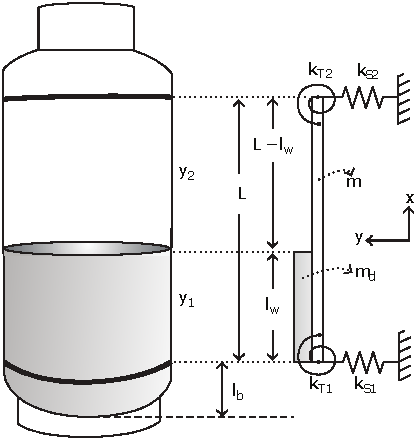
\includegraphics[width=0.45\textwidth]{Chapters/2CHP/Diagrams/mathmodelLPG.pdf}
    \caption{The LPG cylinder filled with liquid, with the mechanical representation of the Euler-Bernoulli beam\cite{wuLiquidLevelDetector2014b}}
    \label{fig:mechanicalmodel}
\end{figure}
\begin{equation} \label{eq:beamEqSimp}
    \begin{split}
        EI\frac{\partial^4y_1}{\partial x^4} + (m + m_d)\frac{\partial^2y_1}{\partial t^2} = 0,\> & \text{for $-l_w \leq x < 0$} \\
        EI\frac{\partial^4y_2}{\partial x^4} + m\frac{\partial^2y_2}{\partial t^2} = 0,\> & \text{for $0 < x < L-l_w$}
    \end{split}
\end{equation}

The variables $y_1$ and $y_2$ correspond to the transverse vibratory displacements o f the beam. Considering that the seam welding's are not ideally clamped or pinned, and the main transverse vibration is restricted between the two boundaries, is assumed that they have small displacements, that will show flexural vibration. This way their model assumes that there is strong linear springs and torsional springs connected at the boundaries. Which obligates to the boundaries conditions to be formulated taking in consideration these factors, where $k_{S1}$, $k_{T1}$ are the linear and torsional springs constants for the lower welding, and $k_{S2}$, $k_{T2}$ are the correspondent spring constants in the upper welding.
\begin{equation} \label{eq:beamEqEv}
    \begin{split}
        At\>x=-l_w \Rightarrow \begin{cases}
            EI\frac{\partial^2y_1}{\partial x^2} = -k_{T1}\frac{\partial y_1(-l_w,t)}{\partial x}\\
            EI\frac{\partial^3y_1(-l_w,t)}{\partial x^3}=-k_{S1}.y_1    
        \end{cases}\\
        At\>x=L-l_w \Rightarrow \begin{cases}
            EI\frac{\partial^2y_2}{\partial x^2} = -k_{T2}\frac{\partial y_2(L-l_w,t)}{\partial x}\\
            EI\frac{\partial^3y_2(L-l_w,t)}{\partial x^3}=-k_{S2}.y_2    
        \end{cases}    
    \end{split}
\end{equation}

At the bottom a circular steel plate is attached to make the cylinder more stable in relation with the ground, this turns it more stable the the upper part, which allow them to conclude that the value of the constants, linear and torsional springs, of the bottom is higher when compared with the upper values, i.e. $k_{S1}>k_{S2}$ and $k_{T1}>k_{T2}$. The continuity and equilibrium condition at the interface of the liquid, inside the cylinder, are:
\begin{equation} \label{eq:beamEqEquilCond}
    \begin{split}
        y_1(0,t) = y_2(0,t),\> y'_1(0,t) = y'_2(0,t) \\
        y''_1(0,t) = y''_2(0,t),\> y'''_1(0,t) = y'''_2(0,t)
    \end{split}
\end{equation}
This conditions allow them to investigate the relation of the normalized frequency ratio $f_r=f/f_0$, considering $f_0$ as the maximum frequency when there is no liquid inside, and the length ratio $l_w/L$ in their experiments.

\subsection{Relation with previous studies}
So far the model presented show very general boundaries conditions, by controlling the variables, the model can be easily compared with models mentioned. Taking that into consideration, a demonstration of this similarities was presented and is the following.
    \todo[inline,color=yellow!40]{Change the word value to another un the following subsubsections(explanation in notes)}
    \todo[inline,color=yellow!40]{Do the changes to close this section}
    %Using value may induce to a defined value, like 0,1,2,3... which is not the case when infinite is used
    \subsubsection{Clamped-free boundaries}
    For this condition, the values of the variables are considered to be $k_{S1}=k_{T1}\approx\infty$ and $k_{S2}=k_{T2}=0$. When \citeauthor{chanFreeVibrationCantilever1995} proposed this model to calculate the frequencies of a cantilever tube, partially filled with liquid mercury, the cantilever was clamped at the bottom and free at the top, and the transverse vibration was generated by using a hammer to knock the tube\ref{fig:clampedfreemodel}. 
    %clamped-free model
    \begin{figure}[!htb]
        \centering
        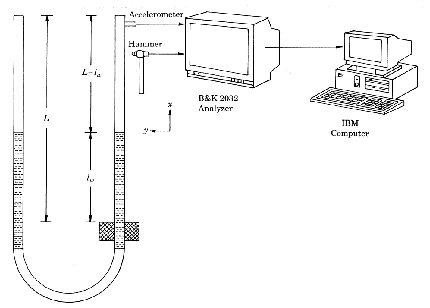
\includegraphics[width=0.45\textwidth]{Chapters/2CHP/Diagrams/clampedfreemodel.pdf}
        \caption{Clamped-Free Model \cite{chanFreeVibrationCantilever1995}}
        \label{fig:clampedfreemodel}
    \end{figure}
    If the values of the variables are replaced in the equation\ref{eq:beamEqSimp} the result of this setup makes the boundaries conditions at their limits, $x=-l_w$ and $x=L-l_w$, to be as shown in \ref{eq:beamEqClamFree}, when comparing the results in the boundaries conditions they verify that they were the same as in \cite{chanFreeVibrationCantilever1995}.
    \begin{equation} \label{eq:beamEqClamFree}
            y_1(-l_w,t) = y'_1(-l_w,t) = y''_2(L-l_w,t) = y'''_2(L-l_w,t)=0
    \end{equation}
    \subsubsection{Pinned-pinned boundaries}
    For this condition, the value of the variables considered is $k_{S1}=k_{S2}\approx\infty$ and $k_{T1}=k_{T2}=0$. In this model, proposed by \citeauthor{chanFREEVIBRATIONSIMPLY1996}, the study is made in a simply supported beam partially load, with distributed mass in both cases\ref{fig:pinnedpinnedmodel}.
    %Pinned-Pinned Model
    \begin{figure}[!htb]
        \centering
        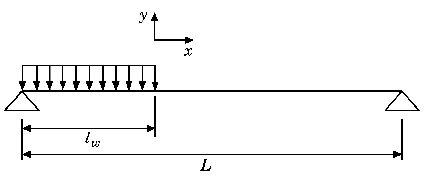
\includegraphics[width=0.45\textwidth]{Chapters/2CHP/Diagrams/pinnedpinnedmodel.pdf}
        \caption{Pinned-Pinned Model\cite{chanFREEVIBRATIONSIMPLY1996}}
        \label{fig:pinnedpinnedmodel}
    \end{figure}
    Once again, if the variables in \ref{eq:beamEqSimp} are replaced with $k_{S1}$, $k_{T1}$, $k_{S2}$ and $k_{T2}$, the result in this setup will also match the boundaries condition\ref{eq:beamEqPinnedx2} at $x=-l_w$ and $x=L-l_w$, obtained in \cite{chanFREEVIBRATIONSIMPLY1996}.
    \begin{equation} \label{eq:beamEqPinnedx2}
        y_1(-l_w,t) = y''_1(-l_w,t) = y_2(L-l_w,t) = y''_2(L-l_w,t)=0
    \end{equation}
    \subsubsection{Clamped-clamped boundaries}
    In this case, the value considered to the variables was $k_{S1}=k_{T1}=k_{S2}=k_{T2}\approx\infty$. This model, proposed by \citeauthor{jacobsContactlessLiquidDetection2005}, with a contactless method to measure the vibration of a opaque capillary tube\ref{fig:clampedclampedmodel}.
    %Clamped-Clamped Model
    \begin{figure}[!htb]
        \centering
        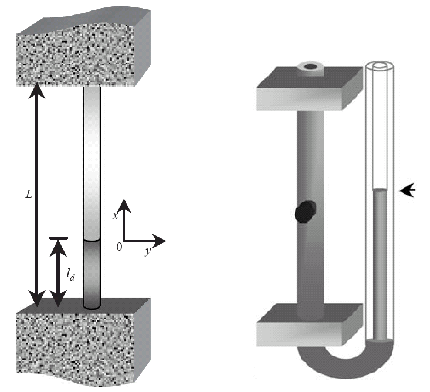
\includegraphics[width=0.45\textwidth]{Chapters/2CHP/Diagrams/clampedclampedmodel1.pdf}
        \caption{Clamped-Clamped Model\cite{jacobsContactlessLiquidDetection2005}}
        \label{fig:clampedclampedmodel}
    \end{figure}
    Following the same path of the previous two, the variables $k_{S1}$, $k_{T1}$, $k_{S2}$ and $k_{T2}$ were once again replaced in \ref{eq:beamEqSimp},and the results obtained\ref{eq:beamEqClampedx2} at their boundaries conditions matched results obtained in \cite{jacobsContactlessLiquidDetection2005}
    \begin{equation} \label{eq:beamEqClampedx2}
        y_1(-l_w,t) = y'_1(-l_w,t) = y_2(L-l_w,t) = y'_2(L-l_w,t)=0
    \end{equation}

    \subsubsection{Relation of Frequency versus Length}
    As a final comparison, the test between the relation of the frequency with the length of the liquid level was executed. For that, different values were attributed to linear and torsional spring variables, to allow the simulation of theoretical curves of the normalized frequency ratio $f_r (f_i/f_0)$ and length ratio $l_r (l_w/L)$. The values for each of the variables were chosen to be large enough to simulate the different boundaries conditions. As expected the results[reference to all images] of \citeauthor{wuLiquidLevelDetector2014b} were very similar with what was previously obtained \cite{chanFreeVibrationCantilever1995}\cite{chanFREEVIBRATIONSIMPLY1996}\cite{jacobsContactlessLiquidDetection2005}, confirming what was mention in the beginning of this section.
    %Theoretical curves
    \begin{figure}[!htb]
        \centering
        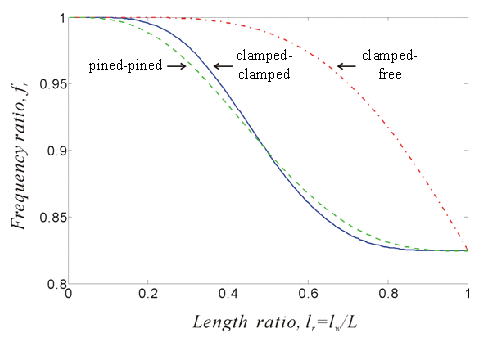
\includegraphics[width=0.45\textwidth]{Chapters/2CHP/Diagrams/theoricalcurve.pdf}
        \caption{Frequency VS Weight - Practical curve obtained by \citeauthor{wuLiquidLevelDetector2014b}}
        \label{fig:theoCurves}
    \end{figure}
    In this relation is important to note that, when the cylinder is almost empty $l_r = 0$ the frequency of the vibration is the highest, in the opposite cases, when the cylinder is full $l_r = 1$ then the vibration frequency is archives the minimum value. 
\subsection{Experimental results}\label{subsec:SOAExpRes}
In the tests perform by \citeauthor{wuLiquidLevelDetector2014b}\cite{wuLiquidLevelDetector2014b}, their setup consisted in a hammer knocking in the lateral surface of the cylinder, that produces the transversal vibration, which is captured by a microphone,processed with a FFT algorithm. By continuously releasing gas and measure the produced vibration, and the correspondent frequency they obtained the following relation: 
%Practical curve obtained
\begin{figure}[!htb]
    \centering
    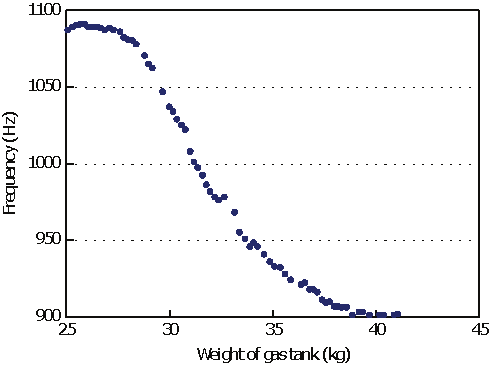
\includegraphics[width=0.45\textwidth]{Chapters/2CHP/Diagrams/weightvsfrequency.pdf}
    \caption{Frequency VS Weight - Practical curve obtained by \citeauthor{wuLiquidLevelDetector2014b}}
    \label{fig:practCurve}
\end{figure}
In the same way of their theoretical simulations, the relation between the vibration frequency and the liquid level(or the length of the liquid) is similar, the highest frequency correspond to the lowest liquid level, and the lowest frequency to the highest liquid level. One thing that is important to refer that is mentioned in their work is, this relation is constant for the different variety of LPG cylinders, but the frequency range of each also varies with the amount of gas that they can store[ref to fig], which means that the device must be adapted to the type of cylinder that is going to be used in. 
%Figures of curves from different bottles
\begin{figure}[ht]
    \centering
    \begin{subfigure}{0.45\textwidth}
        \centering
        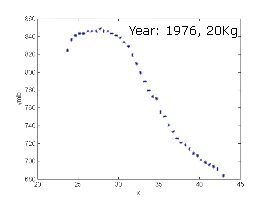
\includegraphics[width=\linewidth]{Chapters/2CHP/Diagrams/g1line.pdf}
        \caption{}
        \label{subfig:g1lines}
    \end{subfigure}
    \begin{subfigure}{0.45\textwidth}
        \centering
        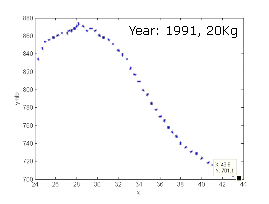
\includegraphics[width=\linewidth]{Chapters/2CHP/Diagrams/g2line.pdf}
        \caption{}
        \label{subfig:g2lines}
    \end{subfigure}
    \begin{subfigure}{0.45\textwidth}
        \centering
        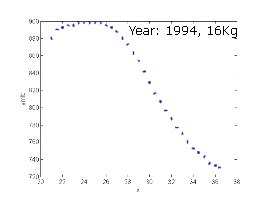
\includegraphics[width=\linewidth]{Chapters/2CHP/Diagrams/g3line.pdf}
        \caption{}
        \label{subfig:g3lines}
    \end{subfigure}
    \begin{subfigure}{0.45\textwidth}
        \centering
        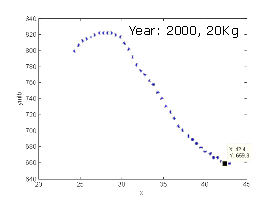
\includegraphics[width=\linewidth]{Chapters/2CHP/Diagrams/g4line.pdf}
        \caption{}
        \label{subfig:g4lines}
    \end{subfigure}
    \caption{Different LPG cylinder to used to compare the relation between Frequency and Weight for different models\citeauthor{wuLiquidLevelDetector2014b}}
     \label{fig:noise}
 \end{figure}
A couple of years latter this work was followed by \citeauthor{wuAnalysisImplementationNoncontact2016a}\cite{wuAnalysisImplementationNoncontact2016a}, were they developed a prototype with the function of measure the frequency of the vibration, and thus the returning the liquid level of the LPG cylinder. The setup used and the test conditions were very similar the the previous work.

\section{Sensors}
To acquire and measure the vibration, the sensors used must work according to the system mechanical or optical principals of vibration. There is a large variety of sensors that ca be used for that purpose, although there isn't a direct method, or sensor, to measure the vibration and they can be either mechanical or optical. The sensors ca be divided in different groups, based on their behavior they can be active or passive, the type of measurement can be either absolute or relative, and there is also some specific characteristics of the signals that differ from the type of sensor, like the frequency range, signal dynamic and the quality of the data acquired. Sensors are divided in contact and non-contact measurement and subdivided in path/displacement, speed/velocity or acceleration.\\
For contact measurements, sensors related to path/displacement can be potentiometric transmitters or Linear Variable Differential Transmitter (LVDT), to speed/velocity it can be applied the principle of electrodynamics or use a seismometer as a sensor and for acceleration the sensors can be piezoelectric, piezo-resistive, resistive or inductive. In non-contact measurements, path/displacement sensors are eddy current sensors, optical sensors and hall sensors, or can be based on the capacitive principle, for speed/velocity is used a Laser-Doppler vibrometer (LDV) and for acceleration isn't possible to measure directly, although it can be derivate from speed/velocity measurement, but induces a lot of noise in the data acquired\cite{SensorsVibrationMeasurement}\cite{VibrationMeasurementVibration2019}.\\
From all the sensors mentioned, is usually used the contact acceleration to measure the vibration. The use of this types of devices is very wide, as well as the type of accelerometer used and usually the application of them is for monitoring equipment in a reliable way in industry.\\ 
Beside the sensors mentioned, one type of sensors that is commonly used to measure vibrations is the accelerometer, the functioning principle can differ from one to another. The basic principle of a accelerometer is similar to a seismometer, from this there are 3 main types, mechanical, capacitive and piezoelectric. The mechanical is the most similar to a seismometer, with a mass attached to a spring, every time that acceleration occurs, just like in seismometer, the mass moves and a pen attached to the mass traces the vibration captured.
%%Insert here a image to illustrate this
% see in https://www.explainthatstuff.com/accelerometers.html  
Although in the case of the accelerometer, doesn't trace with a pen in paper, instead generates a electrical or magnetic signal. A example of this, is a piezoresistive accelerometer, which has a his mass attached to a potentiometer, and the result of the vibration is a voltage change. When a magnetic variation occurs, usually a hall-effect accelerometer is used for that effect.  
Similar to the mechanical, a capacitive accelerometer, has one of the plates attached to the mass, and measures the capacitance variation, the vibration of capacitance is related with the vibration movement. 
%% Insert another image here
In piezoelectric accelerometers, the quartz crystal is attached to the mass, and the deformation in the piezoelectric material produces a voltage change, correspondent to the vibration movement.
%%Insert here
All the type of accelerometers mentioned have one problem, that is the fact that they aren't practical to use in certain application, as an example a small electronic device. For that, is used the so called MEMS (Micro Electro Mechanical Systems) accelerometers, this type of accelerometer is a combination of electrical and mechanical device, mounted on a silicon chip, this is one advantage of this type of accelerometers, the can be very produced in very small sizes, to allows their application in different types of electronic devices. The functioning of this type of accelerometer can be explained quite easily, an electrode is between two other electrodes, there is a air gap between these two and a small insulation to prevent direct contact between the middle electrode and the other two, on the top and the bottom. The middle electrode is connected with a cantilever, rigid enough to hold his position, but flexible enough to allow the move when the accelerometer moves or tilts, the cantilever is connected to outside of the chip, this is used to measure the difference of capacitance between the middle electrode and the electrodes at the top and at the bottom, the capacitance changes every time the middle electrode moves or tilts.\\
 %%insert the image here as a example, get it from https://www.explainthatstuff.com/accelerometers.html

This type of accelerometers brought important advantages, being their low cost and their small size the most important of it. On the other hand, the use of this devices for condition monitoring is restricted to a small bandwidth, restricted to a few kHz, and it cannot be used to in applications that require lower noise over higher frequency ranges \cite{WhatYouNeed}\cite{HowAccelerometersWork2009}.

\clearpage
\printbibliography[heading=subbibliography]
\addcontentsline{toc}{section}{References}